
\documentclass[preprint,12pt]{elsarticle}


\usepackage{amssymb,tabularx,longtable}
\usepackage{geometry,balance}
\usepackage{tabularx}
\newcolumntype{Y}{>{\raggedright\arraybackslash}X}

\usepackage{graphicx,amsmath,booktabs,gensymb}
\geometry{margin=0.75in}


\journal{Journal of building environment}

\begin{document}

\begin{frontmatter}




\title{Ventilation Trade-offs in Retrofitted Municipal Service Buildings: Balancing Indoor Environmental Quality and Energy Efficiency in Hong Kong’s Cooked Food Centers}


\affiliation[inst1]{organization={Department of Architecture, Faculty of Architecture, the University of Hong Kong},
            addressline={Knowles Building}, 
            city={Hong Kong SAR},
            country={China}}


\author[inst1]{Hongshan Guo\corref{cor1}}
\cortext[cor1]{Corresponding author}
\ead{hongshan@hku.hk}
\author[inst1]{Yichun Li\corref{cor2}}
\cortext[cor2]{Corresponding author}
\ead{yichunli@hku.hk}
\author[inst1]{Ying Zhou}
\author[inst1]{Yu Chang}
\author[inst1]{Qingyao, Qiao}
\author[inst2]{Chun Yin Lai}
\author[inst1]{Eric Schuldenfrei}

\affiliation[inst2]{organization={Department of Electrical Engineering, The University of Hong Kong},
            country={Hong Kong SAR}}




\begin{abstract}



Municipal Service Buildings (MSBs) in Hong Kong combine unique architectural heritage with essential civic functions, particularly through their semi-open wet markets known as Cooked Food Centers (CFCs). Recent retrofits have transformed these traditionally naturally ventilated spaces into fully sealed, actively cooled environments, raising concerns about unintended consequences. This study employs snapshot measurements of indoor environmental quality (iEQ), focusing on carbon dioxide ($CO_2$) concentrations, air temperature, relative humidity, particulate matter (PM2.5), and air velocity, to diagnose the ventilation efficiency, thermal comfort, and energy implications of these retrofit strategies. By comparing actively cooled retrofitted buildings against mixed-mode ventilated counterparts during summer conditions, we reveal that retrofitted markets exhibit elevated $CO_2$ concentrations approximately 216 ppm higher on average, along with reduced thermal comfort and increased cooling loads (estimated at 128–255 kW additional demand for a typical market). Our diagnostic approach highlights critical trade-offs inherent in active cooling retrofits and underscores the importance of context-sensitive, hybrid ventilation solutions that better balance occupant comfort, indoor air quality, and energy efficiency.


\end{abstract}



\begin{keyword}

Wet Market \sep Indoor Air Quality

\sep$CO_2$ Measurement\sep Retrofit Strategy \sep Thermal Comfort

\sep Municipal Service Buildings \sep Energy Demand
\end{keyword}
\end{frontmatter}

\section{Introduction}
Hong Kong’s municipal service buildings (MSBs) represent a unique part of the city’s architectural heritage. The MSBs were not just utilitarian structures but became essential communal hubs, serving as “urban living rooms” where social interactions flourished, particularly in dense neighborhoods lacking shared public spaces. Unlike traditional markets in other cities, Hong Kong’s MSBs were uniquely designed to accommodate a variety of public functions, reinforcing their role as key civic anchors. These high-rise structures combine mixed-use spaces and communal areas, with the lower floors dedicated to wet markets—locally known as cooked food centers (CFCs). Traditionally, these CFCs have been semi‑open and naturally ventilated. Built in the 1970s and 1980s across 41 locations\cite{2}, they now serve a population of 7.4 million and are approaching the time for retrofit.

Recent pilot retrofit projects are converting these semi-open CFCs into fully sealed, actively cooled, supermarket-like spaces. Such retrofits may come with unintended consequences. Sealing the building envelope can degrade ventilation performance—evidenced by higher $CO_2$ level, diminish thermal comfort, and increase energy consumption. These unintended costs of modernization raise a critical question: Is enclosing MSBs and CFCs and relying solely on active cooling the most appropriate retrofit strategy? Although many studies have focused on improving indoor environmental quality (iEQ) for occupant comfort, few have used iEQ measurements as a diagnostic tool to assess the design trade-offs in current retrofit strategies. Several previous works have employed $CO_2$ as a proxy for ventilation efficiency\cite{23,24,25}; however, there remains a gap in evaluating how different retrofit designs impact ventilation, thermal comfort, and energy consumption. 

In this study, our main objective is to evaluate the impact of retrofitting CFCs from semi-open, naturally ventilated spaces to fully enclosed, actively cooled environments, focusing on ventilation performance and energy use\cite{5,6}. We capture short bursts of iEQ data in CFCs to diagnose the performance of existing retrofit designs and incorporate a back-of-the-envelope calculation to estimate the extra energy demand resulting from increased cooling loads. It is important to emphasize that our approach is diagnostic rather than performing a traditional before-and-after comparison. Instead of assessing changes post-retrofit, this study uses snapshot measurements to evaluate trade-offs in current retrofit designs, providing insights to refine existing strategies.


Our findings provide quantitative evidence that this retrofit strategy leads to higher $CO_2$ concentrations\cite{7}, poorer thermal comfort and greater energy consumption\cite{8,9}. For MSBs and CFCs, these costs underscore the need to prioritize renovation and refurbishment strategies over comprehensive retrofits. This study holds particular significance, as over 38 MSBs in Hong Kong—along with similar wet markets in Singapore and South Asia—may soon require retrofitting. The remainder of this paper is organized as follows: a background section outlining the retrofit challenge and the use of $CO_2$ as a metric, a methodology section describing our measurement and analysis techniques, and a conclusion that discusses our findings and study limitations.


\section{Background}
\subsection{Evolution and Retrofit Challenge of Hong Kong’s MSBs and CFCs}    
    Hong Kong’s municipal service buildings (MSBs) embody a unique architectural heritage that reflects the city’s rapid post‐war urbanization. Historically, wet markets in Hong Kong were open‐air affairs that relied entirely on natural ventilation—a design well suited to the humid subtropical climate\cite{1}. These early market buildings, constructed predominantly in the 1970s and 1980s, were designed with high ceilings, open layouts, and porous building envelopes that facilitated efficient air movement and heat dissipation\cite{1,2}. Over time, MSBs evolved into mixed‐use complexes that served not only as market spaces but also as communal hubs in densely populated neighborhoods, reinforcing their role as civic anchors\cite{3}.
    
    The introduction of Cooked Food Centers (CFCs) in the 1970s marked a further development in these markets. CFCs were established to improve hygiene standards for street food vendors and were often incorporated into the upper floors of MSBs. This design maintained the benefits of natural ventilation while attempting to manage cooking fumes through mechanical exhaust systems\cite{2,3}. However, as public expectations evolved and the demand for modern indoor environments increased, there has been a growing trend toward retrofitting these semi‐open CFCs. Recent pilot retrofit projects have converted these spaces into fully sealed, actively cooled, supermarket‐like environments\cite{4}.

    Such retrofits, while intended to enhance thermal control and meet stricter hygiene regulations, introduce unintended consequences. By closing the building envelope and relying solely on active cooling, these retrofits reduce the natural ventilation that originally helped dilute contaminants and maintain a comfortable microclimate\cite{4,5}. This shift can lead to degraded ventilation performance, as evidenced by elevated $CO_2$ levels, and an increase in energy consumption due to the additional sensible and latent cooling load required. The challenge for engineers and architects is to balance modernization with the preservation of the cultural and functional essence of these historically vibrant, semi‐open spaces.

\subsection{$CO_2$ as a Diagnostic Tool}
    The COVID-19 pandemic has sharpened our focus on indoor air quality and brought renewed attention to ventilation performance in densely occupied environments. In many studies, $CO_2$ concentration has been used as a practical proxy for ventilation performance and occupant density\cite{17}. In the context of Hong Kong’s MSBs, $CO_2$ measurements are not only indicators of air quality but also reflect the broader impacts of retrofitting—from changes in building enclosure to shifts in social interaction patterns. Rising $CO_2$ levels in sealed, actively cooled CFCs signal that reduced natural ventilation may compromise the spaces’ original function as open, community-oriented environments\cite{8,15}.
    
    Traditional ventilation assessments, which rely on continuous monitoring over long periods, often fail to capture the dynamic nature of semi‑open spaces such as wet markets. In these settings, short‐burst $CO_2$ measurements provide snapshots of how ventilation changes with occupancy and external conditions. When a retrofit converts a semi‑open space into a fully enclosed, mechanically cooled environment, the natural dilution of exhaled $CO_2$ is hindered. Thus, elevated $CO_2$ levels become a diagnostic marker for both diminished air exchange and potential design inferiority in the retrofit strategy\cite{16}. This is especially relevant in MSBs, where the balance between energy efficiency, thermal comfort, and sufficient ventilation is critical. It's important to note that such snapshot measurements capture only a momentary picture of ventilation performance and may be influenced by transient fluctuations in occupancy and outdoor conditions. Consequently, while this approach offers valuable diagnostic insight, supplementing it with longer-term monitoring could further validate the observed trends.
    
    Our study leverages $CO_2$ monitoring as a quantitative method to assess these changes as its concentration has been suggested as a helpful proxy indicator for indoor air quality (IAQ) and ventilation adequacy\cite{persily1997co2}.
    Comparing $CO_2$ concentrations in MSBs with central air conditioning to those in mixed-mode, naturally ventilated markets—alongside control measurements from nearby shopping malls—helps isolate the effects of design modifications on ventilation performance. This approach addresses a significant gap in retrofit evaluations by using $CO_2$ not only as an indoor air quality metric but also as an indicator of the underlying changes in airflow dynamics brought on by modernization efforts\cite{15,17}. In doing so, our method offers a practical tool for diagnosing the unintended costs of closing up these culturally significant, semi‑open spaces.

\section{Methodology}
\label{sec:sample1}
\subsection{Site selection}

Hong Kong currently has a total of 43 Municipal Services Buildings (MSB) spanning across its various districts, with 33 of them containing wet markets. In 2018, the Hong Kong Special Administrative Region Government launched the "Market Modernization Program" and decided to install air conditioning in MSBs to improve the indoor environment\cite{19}. In order to investigate whether these retrofit measures can effectively enhance indoor air quality and create a more pleasant indoor environment, this study examined various MSBs and ultimately selected three of the most representative ones: Aberdeen Municipal Services Building (AB), Kowloon City Municipal Services Building (KL), and Kwun Chong Municipal Services Building (KC), as shown in Figure~\ref{fig:ab,kl,kc}. For each of the targeted MSB building that we identified, we also looked for its control benchmark, a shopping mall within its close proximity as can be seen from Figure~\ref{fig:ab-ref}.

\begin{figure}[h]
    \centering
    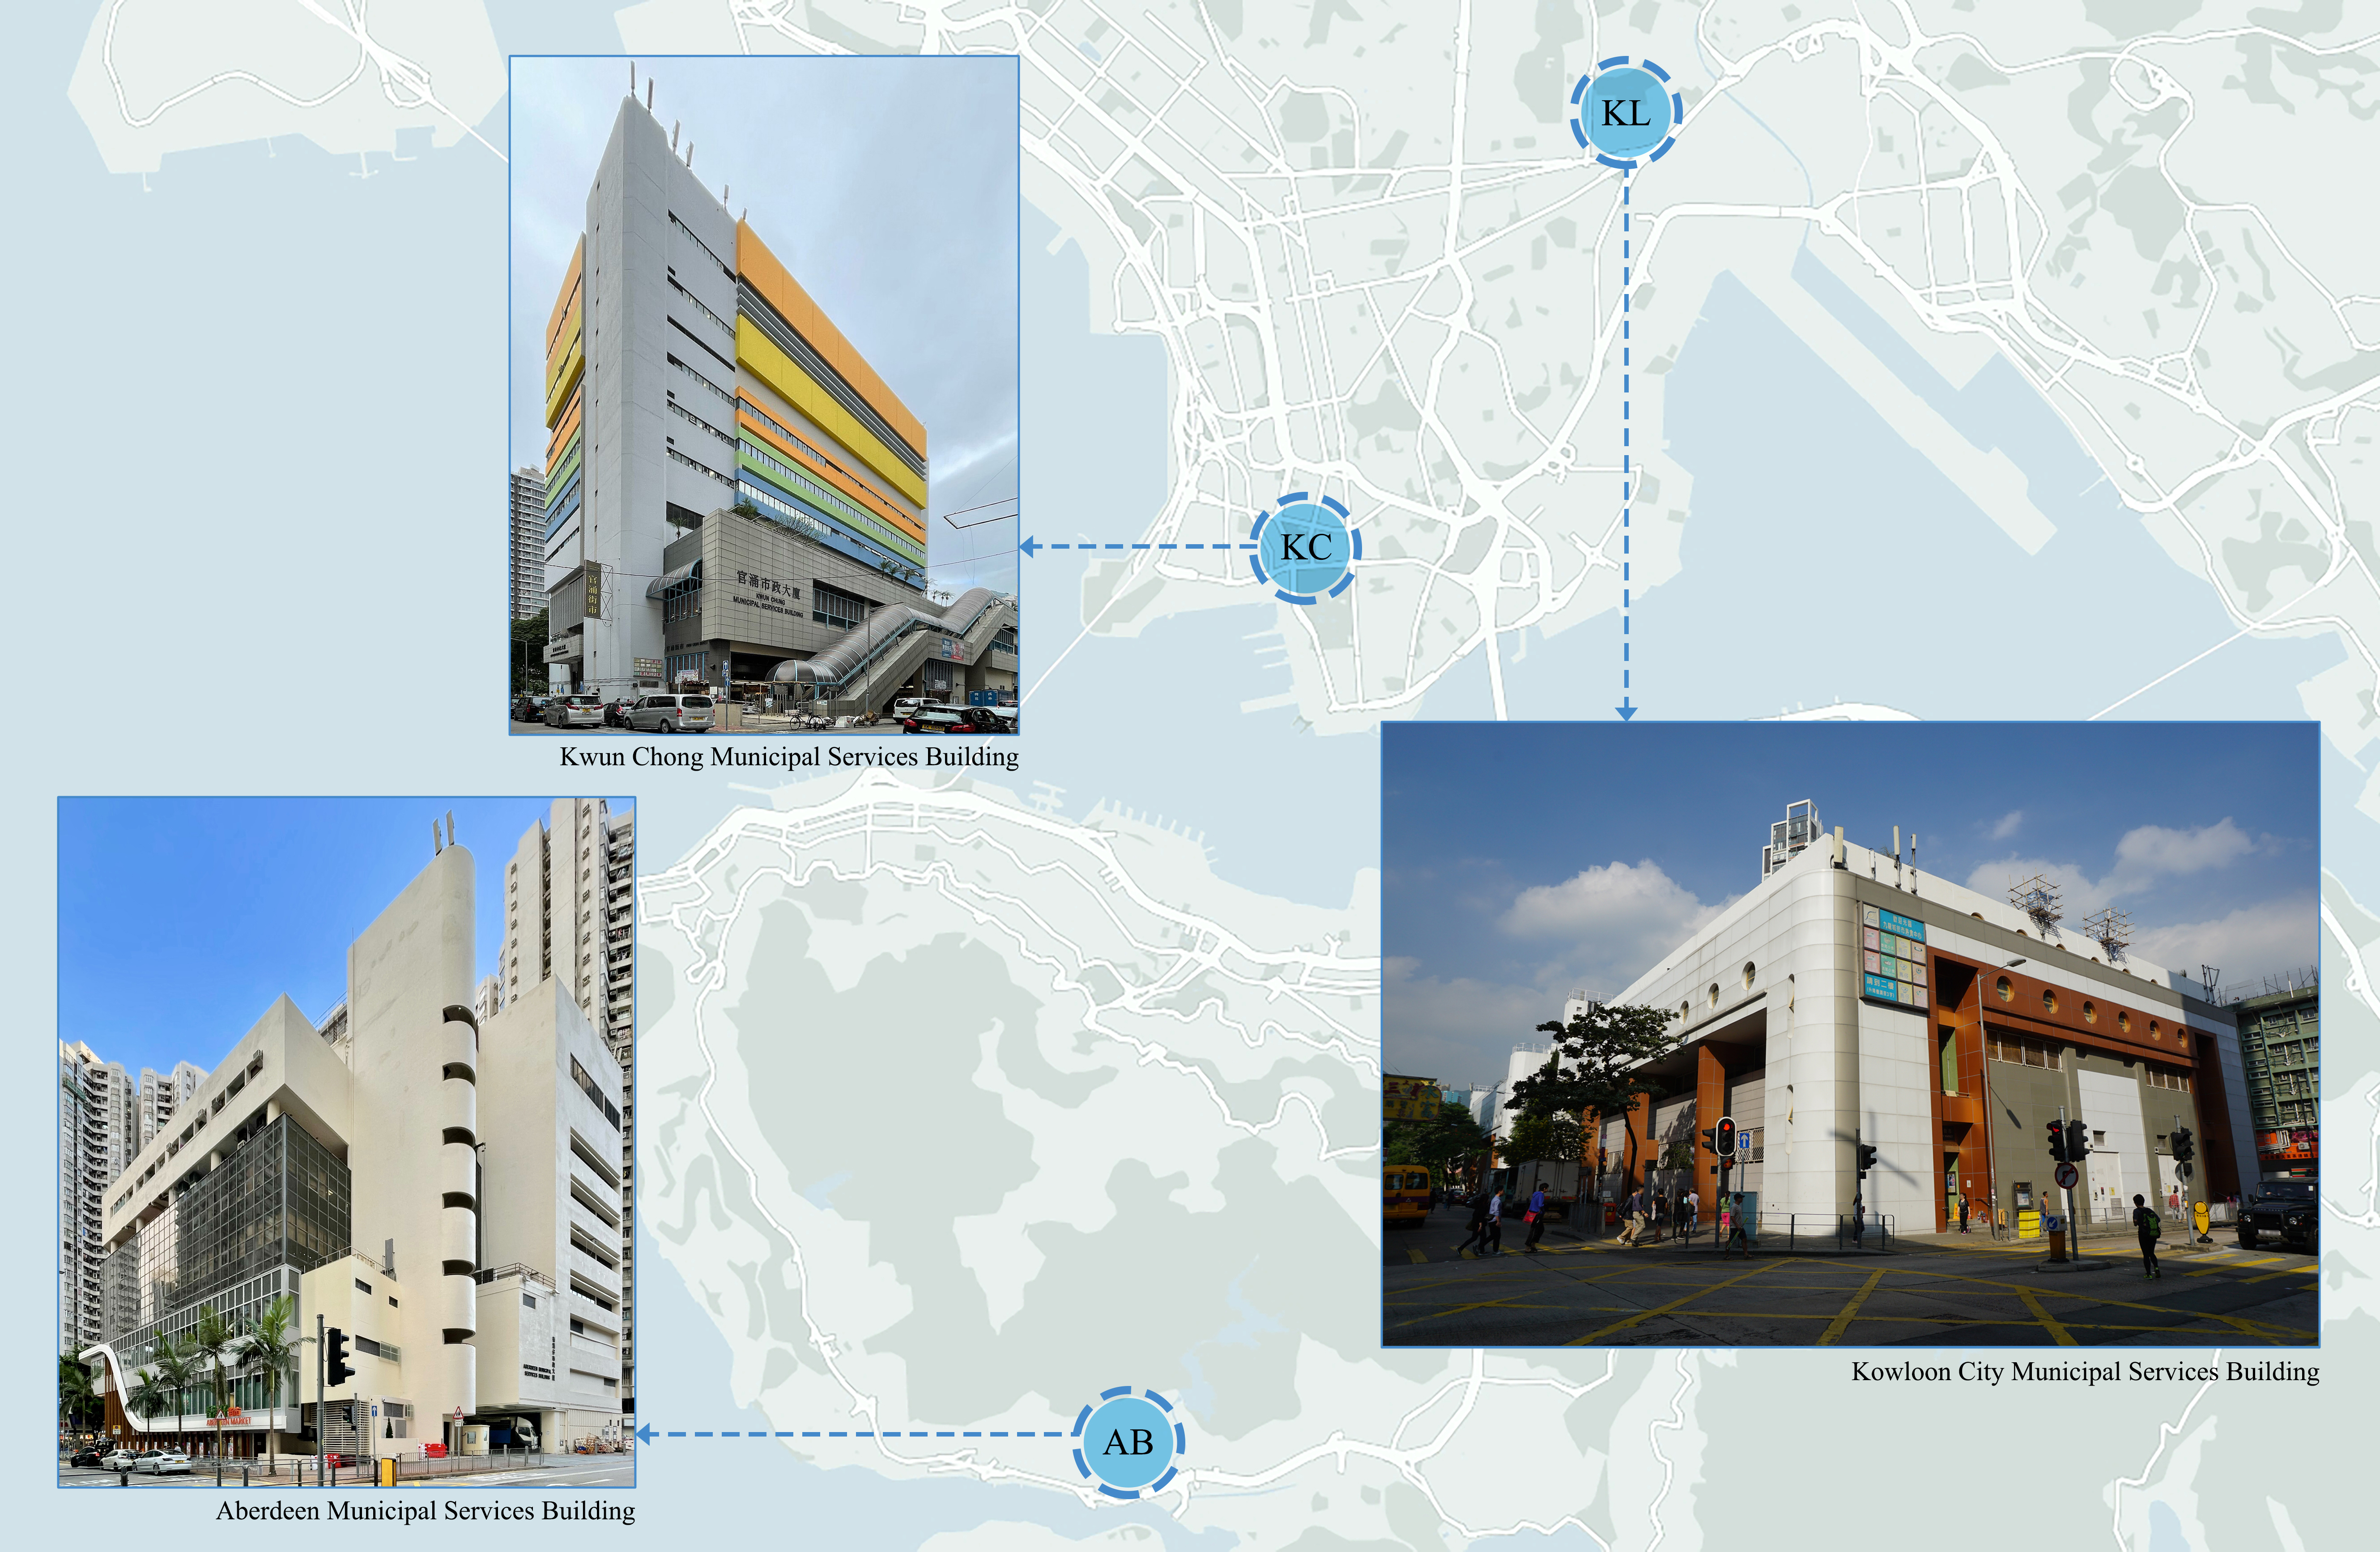
\includegraphics[width=0.7\linewidth]{map3.jpg}
    \caption{Location of Aberdeen MSB, Kowloon City MSB, and Kwun Chong MSB on map}
    \label{fig:ab,kl,kc}
\end{figure}

\begin{figure}[h]
    \centering
    \includegraphics[width=0.5\linewidth]{img/aberdeen_map.png}
    \caption{Location of Aberdeen MSB on map against its reference building closeby}
    \label{fig:ab-ref}
\end{figure}

The Aberdeen Municipal Services Building, established in 1983 as Hong Kong's first, features a wet market, library, offices, sports facilities, and an exhibition center across its seven stories. As shown in Figure~\ref{fig:transition-ab}, the previous building façade was semi-open, facilitating effective indoor air circulation through mixed-mode ventilation and direct openings to the external environment. In contrast, the post-retrofit façade is fully enclosed, with the internal environment now regulated by a newly installed active cooling system. The other two buildings selected—the Kowloon City Municipal Services Building (1988) and the Kwun Chung Municipal Building (1991)—were constructed around the same time as the Aberdeen MSB, sharing similar architectural and functional characteristics. Like the Aberdeen MSB, these buildings utilize a combination of natural and mechanical ventilation for their wet markets. While the Kowloon City MSB is currently awaiting renovation, the Kwun Chung market is nearly abandoned and slated for conversion into an 'urban sports center,' accommodating activities such as rock climbing, breakdancing, and skateboarding.

\begin{figure}[h!]
    \centering
    \scalebox{-1}[1]{\includegraphics[width=0.65\linewidth]{img/Aberdeenb4aft.png}}
    \includegraphics[width=0.7\linewidth]{img/open_to_close_facade.png}
    \caption{From left to right: Aberdeen Cooked Food Center internal (above) images and external (below) before and after its retrofit in 2023.}
    \label{fig:transition-ab}
\end{figure}

\subsection{Experiment Setup} 

    In order to compare the differences in indoor environmental conditions between the retrofitted and unretrofitted MSBs, a total of three rounds of experiments were conducted, collecting environmental parameters at typical locations in the wet market, including air temperature ($T_a$), relative humdity (RH), $CO_2$ concentration, air velocity ($v_a$), barometric pressure ($P_a$), and PM2.5 concentration. The sensors and their corresponding specs can be found in Table ~\ref{tab:protocols} below. As the floor plans from all MSB markets are a part of the government records whose copies are not made available for download but rather for read access only, we only obtained floor plan that has a high-enough resolution for the Aberdeen market from an architectural archive as in Figure~\ref{fig:ab-floorplan}, where each of the gray dots point to one of the four locations measured for each round on the two stories covered.

    \begin{figure}[h!]
        \centering
        \includegraphics[width=0.55\linewidth]{013669_001(cy_update).jpg}
        \caption{Market floor plan of the Aberdeen (AB) market with locations measured on Level 3 (Level 2 at the same location) as retrieved from M+ Archives\cite{dennis_lau__ng_chun_man_architects__engineers_hk_limited_level_1979}}
        \label{fig:ab-floorplan}
    \end{figure}
    
\begin{table}[htbp]
\centering
\resizebox{\textwidth}{!}{%
\begin{tabular}{@{}lccc@{}}
\toprule
\textbf{Parameter}       & \textbf{Round I}                                                              & \textbf{Round II}                                                              & \textbf{Round III}                                                          \\ \midrule
\textbf{Date}            & Mar 26, 2024                                                                & Oct 17, 2024                                                                & Oct 23, 2024                                                                \\
\textbf{Time}            & 2:00--4:00 PM                                                                & 5:00--8:00 PM                                                                & 3:00--5:00 PM                                                                \\
\textbf{Sensor Setup}    & Arduino kit: SCD41, DHT22, FS3000, BME280                                    & Improved kit: SCD41, BMP380, SDP810, SEN54                                      & Backpack sensors: SCD41, BMP380, SDP810, SEN54                                \\
\textbf{Height (m)}      & 1.2                                                                         & 1.5 (Tripod)                                                                 & 1.0--1.2 (Backpack)                                                          \\
\textbf{Duration X Locations}        & 15 minutes x 8                                                                  & 15 minutes x8                                                                 & 10 minutes x 8                                                                  \\
\textbf{Monitored Parameters} & \(CO_2\), \(T_a\), RH, \(v_a\), Pa                                         & \(CO_2\), \(T_a\), RH, PM2.5, Pa                                               & \(CO_2\), \(T_a\), RH, PM2.5, Pa                                               \\
\textbf{Buildings Covered}    & Aberdeen, Kwun Chong                                                    & Aberdeen, Kowloon City, Kwun Chong                                             & Aberdeen, Kowloon City, Kwun Chong                                                       \\ \bottomrule
\end{tabular}%
}
\caption{Experiment Rounds and Measurement Protocols over three days of measurements..\\ \textbf{Abbreviations:} \(T_a\) = air temperature, RH = relative humidity, \(v_a\) = air velocity, Pa = air pressure, PM2.5 = particulate matter (particles $\leq 2.5\,\mu\text{m}$).}
\label{tab:protocols}
\end{table}

    The sensing of $CO_2$, in the meantime, saw itself developing much further from expensive and slow-responding and expensive NDIR (non-dispersive infrared) "photometric" sensors to cheaper alternatives that are photoacoustic. Not only has these new alternatives pushed the price down to monitor $CO_2$ levels, the settling time has also drastically decreased from several days\cite{emmerich2005} to tens of minutes\cite{fisk2008} to as fast as 1min only\cite{sensirion2021,sensirion_scd4x_nodate}. Comparing the two technology, NDIR sensors typically settle faster since the measurement of $CO_2$ is in open-air optical path rather than relying on gas diffusion into a sealed chamber. Nonetheless, for low-cost sensors, low-cost variants like SCD41 (as this study deploys) has high accuracy within 400-5000 PPM for $CO_2$, is compliant with California Title24, RESET and WELL standards for buildings\cite{senseair2020,sensirion2021}. With its compatibility to common IAQ/building standards, we selectedc the SCD41 sensor due to its lower cost (well below 50 USD when purchased in bulk), reasonable response time and compact form factor to work with the developer boards.

    Four SCD41 sensors were first subjected to an initial round of calibration in an open environment, followed by a consistency verification in a sealed office environment, to ensure the accuracy and comparability of measurement data\cite{28}. This step was completed in the Lung Fu Shan area at a location characterized by good air circulation due to its elevation on Hong Kong Island (approximately 110 meters above sea level). For the calibration, the necessary preparations included the SCD41 sensors, a standard $CO_2$ sensor, and laptop supporting WebSerial. Initially, the SCD41 sensors were connected to the laptop, and the corresponding serial device was selected and connected via the WebSerial webpage. The "nRF Connect for Mobile" application was then used to monitor $CO_2$ concentration to ensure continuous reading is coming in real-time. We aspired to avoid obstruction of an outer casing so opted for socket-ready IoT board as shown in Figure~\ref{fig:equipment-setup} where no additional structure interferes with the measurements from $CO_2$ and other iEQ sensors.

    \begin{figure}[h]
        \centering
        \includegraphics[width=0.5\linewidth]{img/setup.png}
        \caption{Sensors hooked up to IoT board as getting prepared for initial round of measurements.}
        \label{fig:equipment-setup}
    \end{figure}
    
    For instance, when the standard sensor indicated a $CO_2$ concentration of 400 ppm\cite{29}, the command “cal\_$CO_2$ 400” was entered into the WebSerial application to initiate the calibration. Upon completion, the sensor returned a confirmation of successful calibration. Post-calibration, four SCD41 sensors along with the standard $CO_2$ sensor were placed together in a sealed plastic bag to further verify the accuracy of their readings. In this enclosed environment, the sensor readings gradually converged towards the standard sensor's value, ultimately maintaining a deviation within 20 ppm. This step ensured the accuracy of the sensors after calibration. 
    
    Subsequently, another calibration was performed in a sealed office environment to validate the consistency of the sensor readings. Four SCD41 sensors and the standard $CO_2$ sensor were prepared, and a sealed office space was selected to maintain stable environmental conditions during the test. The sensors were placed in the same location within the office to ensure they were exposed to the same air condition.The sensors were then allowed to operate for an extended period, with continuous measurement data being recorded. A comparison of the readings from the four SCD41 sensors using the mobile application "nRF Connect for Mobile" revealed that the sensor readings were consistent, confirming the comparability of the experimental results. 

\subsection{Measurement}
    
    All sensors from Table~\ref{tab:protocols} were configured to sample data continuously during each measurement session. In Round I, data were collected at a rate of 1 sample per second. In Rounds II and III, the sensors recorded data every 10 seconds; effectively, these rounds produced data that are averaged over 10-second intervals. To ensure consistency across all rounds, the Round I data were post-processed by averaging over 10-second intervals, thereby harmonizing the sampling methodology. Moreover, each location was monitored for a fixed duration—15 minutes in Rounds I and II, and 10 minutes in Round III—with an additional 5-minute outdoor measurement taken prior to each session. These measures were implemented to minimize variability due to differences in sampling rates and to ensure that the observed differences in $CO_2$ and other iEQ metrics are attributable primarily to the building system design rather than to measurement timing or occupancy fluctuations.
    
    The first round of the experiment took place on March 26, 2024, from 2:00 to 4:00 p.m., with the highest temperature recorded at 28°C. Utilizing a set of sensors from an Arduino kit\cite{30}, including the SCD41 $CO_2$ sensor ($\pm$50ppm), DHT22 temperature and RH sensor ($\pm$0.5°C, $\pm$2\% ), FS3000-1005 air speed sensor (5\%), and BME280 $P_a$ sensor ($\pm$0.1kPa), measurements were taken at a height of 1.2 meters\cite{31}. At each location, sensors were activated, data recorded, then deactivated before moving on. This round of the experiment covered 17 locations within four buildings, including the Aberdeen and Kwun Chong MSBs and their adjacent shopping malls.
    
    As the initial round of experiment only revealed the relationship between the indoor and outdoor environment within the CFC buildings identified, we conducted two additional rounds of experiments respectively on October 17, 2024, from 5:00 to 8:00 p.m., and on October 23, 2024, from 3:00 to 5:00 p.m., where highest air temperatures reached 30°C and 27°C. These rounds utilized an improved sensor kit, measuring temperature, relative RH, and $CO_2$ with the SCD41 sensor ($\pm$50ppm, $\pm$0.5°C, $\pm$2), differential $P_a$ and air speed with the SDP810 sensor ($\pm$500Pa), barometric $P_a$ with the BMP380 sensor ($\pm$0.5hPa), and PM 2.5 with the SEN54 sensor ($\pm$10\%). Upon inspecting the data collected, we noticed Kwun Chong, despite being very well-ventilated did not have as high a population density as was seen in Aberdeen against its control case shopping malls, hence we proceeded to include a third market, Kowloon City into our subsequent measurements.
    
    In the second round, sensors were fixed on tripods at a height of 1.5 meters, while in the third round, they were placed on the side of a backpack at a height of approximately 1 to 1.2 meters\cite{32}. Each location was monitored for 15 minutes, with the sensors continuously recording data. In the third round, the time spent at each measurement location was reduced to 10 minutes, and outdoor climate conditions were measured for 5 minutes outside each building before the experiment began.
    
    The latter two rounds included the Kowloon City MSB, measuring a total of 24 points within six buildings. These locations encompassed areas with significant differences in air quality within each building\cite{33}, such as entry and exit points, air conditioning vents or fans at the lowest levels, and areas with the most or least crowded populations. These measurements allowed for the observation of significant differences in $CO_2$ concentration within the buildings.
    
\subsection{Post-Processing of Data Collected}
    Once the measurement was done, we consolidated the measurement records from all three rounds of measurements into a larger dataset. We also created additional columns with known traits such as measurement of the outdoor environment (`outdoor') as well as the state of movement of the occupants (`moving'). Any transient fluctuations in $CO_2$ readings observed during the initial 30 seconds of sensor activation were excluded from the analysis to ensure that only stable, representative data were used. Meanwhile, The settling effect is a known phenomenon in field measurements, where sensor readings initially fluctuate before stabilizing\cite{fradenHandbookModernSensors2016}. By carefully calibrating the sensors and excluding transient data from the analysis, we ensured that only stable, reliable iEQ measurements were used to diagnose ventilation performance. We also mapped the system type of various buildings to two different types: `mixed' and `active', pointing to respectively buildings that are equipped with either almost all-natural ventilation (with a slight enhancement from mechanical ventilation) or active cooling system i.e. air-conditioning. 
    
    To quantify the additional energy demands introduced by retrofitting semi-open markets into fully sealed, actively cooled environments, we performed simplified cooling load estimations following standard HVAC calculation methods (ASHRAE guidelines). Specifically, we estimated sensible and latent cooling loads using assumptions of air changes per hour (ACH = 6), an assumed ceiling height (3 meters), temperature differences ($\Delta T$ ranging from 4–8 K), and humidity ratio differences ($\Delta \omega $ from 0.005–0.010 kg water/kg air). Detailed analytical calculations, sensitivity considerations, and resulting energy estimates are comprehensively presented and discussed in the discussion section of this paper. As most of the calculation are rule-based following explicit equations, they are kept in the discussions section for coherence.

\section{Results}
\subsection{Indoor Environmental Measurements ($CO_2$,$T_a$, RH, PM2.5 and Air velocity)}
We consolidated indoor environmental quality (IEQ) measurements collected across three rounds of experiments conducted in three representative Municipal Service Buildings (MSBs): Aberdeen (AB), Kowloon City (KL), and Kwun Chong (KC). Specifically, we report measured concentrations of carbon dioxide ($CO_2$), air temperature ($T_a$), relative humidity (RH), particulate matter (PM2.5), and air velocity ($v_a$). Figure~\ref{fig:TaRHva} summarizes the measured Ta, RH, and va, showing clear variations between buildings utilizing active cooling and those employing mixed-mode ventilation. Notably, actively cooled buildings exhibited significantly lower temperatures and air velocities, with Aberdeen displaying consistently lower air velocity and higher humidity relative to Kowloon City and Kwun Chong.


    \begin{figure}[h!]
        \centering
        \includegraphics[width=\linewidth]{img/TaRHva.png}
        \caption{Violinplot of air temperature, relative humidity and air velocity across multiple locations and rounds of experiments (KL was not measured in Round I so is missing across all three plots.)}
        \label{fig:TaRHva}
    \end{figure}

The resulting Figure~\ref{fig:TaRHva} summarizes the measured air temperature, relative humidity and air velocity across the three MSBs. Air temperature measurements indicate a distinct cooling effect in actively cooled environments, with temperatures consistently lower than outdoor conditions, while buildings relying on mixed-mode ventilation (e.g., KC and KL) exhibited higher and more variable indoor temperatures. Relative humidity showed greater variability, particularly influenced by occupancy and activities within each building (e.g., cooking processes), with Aberdeen generally maintaining higher humidity levels potentially driven by their cooling system of choice. Air velocity measurements further reveal notable differences: Aberdeen consistently presented the lowest velocities, suggesting less air movement, whereas Kowloon City and Kwun Chong demonstrated higher and more variable air velocities indicative of more dynamic airflow patterns.

\begin{figure}[h!]
    \centering
    \includegraphics[width=0.5\linewidth]{COST_CO2.png}
    \caption{$CO_2$ Meausred at various locations across system types during all three rounds of measurements in Density Plot (top) and Scatter Plot  against air velocity (Bottom).}
    \label{fig:$CO_2$-types-meas}
\end{figure}


Moving on to our next parameter of interests, $CO_2$, Figure~\ref{fig:$CO_2$-types-meas} presents the measured $CO_2$ concentrations across various locations and rounds of measurements, comparing the three primary test buildings (AB, KC, KL) and their corresponding reference buildings (REF\_AB, REF\_KC, REF\_KL). In the unit of X axis of upper plot, each colored curve represents the distribution of $CO_2$ within each building, revealing distinct concentration patterns. Notably, the Aberdeen (AB) building shows a narrower and distinctly shifted peak, reflecting consistently elevated $CO_2$ levels relative to Kowloon City (KL) and Kwun Chong (KC). Quantitatively, the average $CO_2$ concentration within the retrofitted Aberdeen building is approximately 216 ppm higher than its mixed-mode ventilated counterparts. The lower scatter plot additionally compares measured $CO_2$ concentrations against air velocities ($v_a$), indicating Aberdeen’s $CO_2$ concentrations generally cluster in higher ranges with comparatively lower air velocities than KC and KL.


We also compared the particulates level differences across different buildings and locations/rounds of measurements as plotted out in Figure~\ref{fig:PMVals}. Despite different types of reference building systems, it is clear that the particulates level within the CFCs fluctuates across a much wider range across various sizes from PM 1.0 through PM 10.0, amongst which we picked PM2.5 to plot in Figure~\ref{fig:PMVals} as a well-recognized Particulate Matter metric.
    
    \begin{figure}[h!]
    \centering
    \includegraphics[width=0.85\linewidth]{img/air_pm.png}
    \caption{Scatterplot of PM2.5 levels (PPM) versus air velocity. Marker colors indicate system type, with blue markers representing mixed-mode ventilation (KC, KL) and black markers representing measurements from active cooling systems (AB)}\label{fig:PMVals}
    \end{figure}

Observing Figure~\ref{fig:PMVals}, it clearly shows actively cooled environments (AB) exhibit higher variability and generally elevated PM2.5 concentrations, especially at lower air velocities. In contrast, mixed-mode ventilation systems (blue markers) typically demonstrate lower PM2.5 concentrations, coupled with relatively higher and more variable air velocities. This visual comparison underscores distinct differences in particulate matter handling between the two ventilation system types, with actively cooled systems frequently showing elevated PM2.5 levels despite stable, lower air velocities.

To better understand the relationship between different environmental parameters and how well they represent the ventilation effectiveness, we compared within our collected data their perason correlation coefficient as well as $R^2$ in the following Figure~\ref{fig:trianglescatter}.

\begin{figure}[h!]
    \centering
    \includegraphics[width=0.45\linewidth]{img/aircorr.png}\includegraphics[width=0.55\linewidth]{img/co2scatter.png}
    \caption{Pearson Correlation Coefficient of relevant iEQ measured against air velocity (left) and scattered plot of them against air velocity with linear regression lines (right).}
    \label{fig:trianglescatter}
\end{figure}

Across all measured parameters, carbon dioxide ($CO_2$) demonstrated the clearest inverse relationship with air velocity, as shown in both the scatter plots and the correlation matrix in Figure~\ref{fig:trianglescatter}. $CO_2$ concentrations exhibited a moderately negative correlation with air velocity (r = -0.306), translating to an $R^2$ of 0.094—substantially higher than other environmental variables such as PM2.5 ($R^2$ $\approx$ 0.026), PM1.0 ($R^2$ $\approx $ 0.026), or the VOC index ($R^2$ $\approx$ 0.014). These patterns suggest that air velocity, as a proxy for natural ventilation, has a more consistent and interpretable effect on $CO_2$ dilution than on pollutant concentrations, which tend to vary based on source, filtration, and other environmental factors.

This result affirms $CO_2$’s value as a primary diagnostic indicator for ventilation effectiveness in semi-public environments. Unlike particulate matter, which may reflect localized emissions or filtration dynamics, $CO_2$ concentrations are more directly linked to human occupancy and air exchange rates. The higher degree of statistical alignment between $CO_2$ and air velocity allows us to quantitatively assess the cost of reduced ventilation in retrofitted spaces—specifically, the buildup of exhaled air due to diminished airflow. This relationship forms the basis for interpreting ventilation efficiency and energy trade-offs in subsequent analyses.

\subsection{Calculated Parameters: From Heat Stress to Thermal Comfort}

Beyond wet bulb temperature, the first actual indice of thermal stress that we want to examine is UTCI, which provides us a quantitative measure to how the thermal stress is being experienced by the occupants through the measured space\cite{35}. One of its core benefit is that it stretches across multiple heat stress categories from the numerical calculation fo the temperature-like UTCI values. The environment that we are investigating also do not go beyond the acceptable range of environmental conditions for UTCI, as the CFC centers do not have extreme values that tend to skew the UTCI calculation due to numerical instability in contributing to the polynomial equations in computing UTCI values. On that front, we leveraged the pythermalcomfort package\cite{36}, which allows for calculating UTCI through empirical formulations and regression models in calculating UTCI values.

\begin{figure}[h!]
    \centering
    \includegraphics[width=0.95\linewidth]{img/DIST_heatstress_Tw_subplots.png}
    \caption{Heat Stress Category Experience expressed by UTCI shown across buildings and their corresponding references across all three rounds of measurements.}
    \label{fig:heatstress-breakdown}
\end{figure}

Figure ~\ref{fig:heatstress-breakdown} presents distributions of calculated wet bulb temperatures across the three Municipal Service Buildings (Aberdeen, Kowloon City, and Kwun Chong) and their adjacent reference buildings. Wet bulb temperatures are categorized according to established heat stress levels. That is moderate, strong, very strong according to the UTCI classes they below to in order to better understand the resulting wet bulb glob temperature's meaning, allowing for highlighting variations in occupant heat stress experiences. Aberdeen displays distinctly lower wet bulb temperatures compared to Kowloon City and Kwun Chong, with most measurements categorized within lower heat stress ranges. In contrast, Kowloon City and Kwun Chong exhibit consistently higher wet bulb temperatures, frequently categorized within “strong” or “very strong” heat stress ranges. Notably, adjacent reference buildings exhibit systematically lower wet bulb temperatures than their corresponding market buildings, suggesting differences in microclimatic conditions within closely situated building environments. 




\begin{figure}[h!]
    \centering
    \includegraphics[width=0.95\linewidth]{COST_COMF.png}
    \caption{Predicted Mean Vote, Percentage of People Dissatisfied and Physiological Equivalent Temperature Calculated across all locations measured.}
    \label{fig:pmv3}
\end{figure}

Similarly, Figure~\ref{fig:pmv3} summarizes calculated thermal comfort indices—Predicted Mean Vote (PMV), Percentage of People Dissatisfied (PPD), and Physiological Equivalent Temperature (PET) across all measurement locations and rounds. Aberdeen, the actively retrofitted building, is highlighted separately alongside mixed-mode ventilated buildings (KC, KL) and reference actively cooled buildings. The PMV values for Aberdeen frequently exceed recommended thresholds ($\pm$0.5), indicating occupants experience conditions beyond optimal thermal comfort ranges. Similarly, Aberdeen’s PPD consistently surpasses the recommended dissatisfaction limit (10\%), suggesting higher potential occupant dissatisfaction relative to mixed-mode ventilated buildings. Additionally, PET values indicate Aberdeen’s indoor thermal conditions frequently fall outside the recommended comfort band (26–28$\degree C$), typically skewed towards lower PET values, indicating cooler indoor conditions relative to its mixed-mode counterparts.


\section{Discussions}
\subsection{Ventilation and Indoor Air Quality}
Our results showed significant differences in ventilation effectiveness and indoor air quality between actively cooled and mixed-mode ventilated Municipal Service Buildings (MSBs). The consistently elevated $CO_2$ concentrations observed in Aberdeen’s retrofitted building suggest a clear reduction in ventilation efficiency, attributable to the sealing of previously semi-open facades. Specifically, the observed mean increase in $CO_2$ concentrations (~216 ppm higher than mixed-mode counterparts) underscores a critical trade-off associated with modern retrofit strategies that prioritize thermal control over natural ventilation.

Furthermore, the lower air velocities measured within actively cooled environments, particularly Aberdeen, further support the notion that sealing building envelopes hampers natural air circulation, reducing the dilution of indoor contaminants and occupant-generated $CO_2$. The combined effect of elevated $CO_2$ and reduced air velocities points towards compromised indoor air quality and potential implications for occupant comfort and health. In contrast, the mixed-mode ventilated MSBs (Kowloon City and Kwun Chong) demonstrated significantly better ventilation performance, characterized by lower $CO_2$ concentrations and higher, more variable air velocities, which are indicative of improved air exchange and dilution of indoor pollutants.

The particulate matter (PM2.5) data further reinforces these observations. Actively cooled systems exhibited elevated and more variable particulate concentrations at lower air velocities, suggesting limited effectiveness in filtering or removing indoor pollutants when natural airflow is restricted. Mixed-mode systems, conversely, maintained lower particulate concentrations alongside higher air velocities, illustrating the inherent advantage of hybrid ventilation approaches in promoting healthier indoor air quality. These findings collectively underscore the necessity of reevaluating fully enclosed retrofit strategies for traditionally semi-open municipal buildings, advocating instead for tailored, hybrid solutions that integrate controlled natural ventilation alongside targeted active systems to better balance indoor air quality, occupant comfort, and energy efficiency.

Our decision to prioritize $CO_2$ as the diagnostic indicator of ventilation effectiveness is supported both conceptually and empirically. Unlike PM2.5 or VOC concentrations, which are influenced by localized activities, external pollutants, and filtration strategies, $CO_2$ provides a more stable and direct signal of occupancy-driven air quality and ventilation performance. This is reinforced by our comparative analysis: $CO_2$ exhibited the strongest and most consistent inverse relationship with air velocity among all measured parameters ($R^2$ $\approx$ 0.094), substantially exceeding the explanatory power of other metrics. This suggests that $CO_2$ not only reflects the dilution of exhaled air but also reliably captures the cumulative impact of enclosure and airflow reduction—central to understanding the consequences of retrofit strategies that diminish natural ventilation.
\subsection{Thermal Comfort Implications}
The thermal comfort indices calculated in this study (PMV, PPD, and PET) reveal important insights regarding the occupant experience in retrofitted versus mixed-mode ventilated Municipal Service Buildings (MSBs). While active cooling systems have been widely adopted under the assumption of improved occupant comfort, our findings indicate a nuanced outcome. Specifically, the retrofitted Aberdeen building, despite achieving lower indoor air temperatures, frequently registered PMV values beyond the recommended comfort range (±0.5), signifying that occupants experience conditions perceived as either excessively cool or uncomfortable.

The elevated PPD values in Aberdeen further support this observation, consistently exceeding the recommended dissatisfaction threshold of 10\%. This indicates that despite the introduction of active cooling intended to enhance thermal comfort, a substantial proportion of occupants may remain dissatisfied. This dissatisfaction likely arises from issues such as excessive cooling or inappropriate humidity management, both characteristic outcomes associated with sealing previously semi-open environments and relying solely on mechanical conditioning.

Furthermore, the Physiological Equivalent Temperature (PET) results corroborate these concerns. Aberdeen frequently exhibited PET values below recommended comfort thresholds (26–28$\degree C$), suggesting a tendency towards overcooling, which contrasts sharply with mixed-mode buildings like Kowloon City and Kwun Chong. The elevated thermal stress levels in Kowloon City and Kwun Chong, indicated by higher wet bulb temperatures, present a contrasting scenario in which insufficient active cooling or limited airflow management results in uncomfortable conditions.

Taken together, these findings highlight that fully sealed retrofit strategies, while achieving lower air temperatures, do not necessarily translate into improved occupant comfort. Instead, they may inadvertently produce environments perceived as excessively cool or inadequately balanced regarding humidity and airflow. This underscores the importance of adopting context-specific retrofit strategies, such as hybrid ventilation systems, that maintain natural airflow and provide more precise thermal regulation, ultimately enhancing occupant comfort while avoiding unnecessary energy expenditure.

\subsection{Back-of-the-Envelope Estimation of Cooling Loads}\label{seg:energy}

It is important to note that the following calculations are back-of-the-envelope estimations based on simplified, static rules using standard HVAC equations. These estimates are intended solely as a diagnostic tool to provide an order-of-magnitude understanding of additional cooling loads. They do not incorporate transient effects or detailed dynamic simulations that a full computational model would address. Nonetheless, to quantify the additional energy required by a retrofit that converts a semi-open, naturally ventilated Cooked Food Center (CFC) into a fully sealed, actively cooled environment, we estimate both the sensible and latent cooling loads. We assume that the retrofitted system is designed to meet a minimum ventilation requirement of $ACH$ (air changes per hour) as prescribed by local regulations.

For a given CFC with floor area $A$ (in m$^2$) and an assumed ceiling height $h$ (in m), the building volume is
\[
V = A \times h.
\]
The required ventilation flow rate $Q$ (in m$^3$/s) is then given by
\[
Q = \frac{ACH \times V}{3600}.
\]
Multiplying by air density $\rho$ (approximately 1.2 kg/m$^3$) yields the mass flow rate:
\[
\dot{m} = \rho\, Q.
\]

The sensible cooling load $Q_{\text{sens}}$ (in watts) is calculated as
\[
Q_{\text{sens}} = \dot{m}\, c_p\, \Delta T,
\]
where $c_p$ is the specific heat capacity of air (approximately 1.005 kJ/(kg$\cdot$K)) and $\Delta T = T_{\text{out}} - T_{\text{set}}$ is the temperature difference between the outdoor air temperature $T_{\text{out}}$ and the target indoor temperature $T_{\text{set}}$ (assumed to be 24$^\circ$C).

The latent cooling load $Q_{\text{lat}}$ is estimated by
\[
Q_{\text{lat}} = \dot{m}\, h_{fg}\, \Delta \omega,
\]
where $h_{fg}$ (approximately 2500 kJ/kg) is the latent heat of vaporization and $\Delta \omega$ is the difference in humidity ratio between the outdoor and desired indoor conditions. In our calculations, we assume $\Delta \omega$ to range from 0.005 to 0.010 kg water/kg air following ASHRAE Standard 62.1's specification on ventilation‑load calculation procedure\cite{ashrae2022}.

Thus, the total additional cooling load is
\[
Q_{\text{total}} = Q_{\text{sens}} + Q_{\text{lat}}.
\]

For our estimates, we assume a uniform ceiling height $h = 3$ m and $ACH = 6$. The floor areas for the three CFCs are as follows:
\begin{itemize}
    \item \textbf{Aberdeen}: $A = 1288$ m$^2$
    \item \textbf{Kowloon City}: $A = 340$ m$^2$
    \item \textbf{Kwun Chong}: $A = 3260$ m$^2$
\end{itemize}

By substituting these values into the above equations and applying a range for $\Delta T$ (e.g., 4--8 K) and $\Delta \omega$ (0.005--0.010 kg/kg), we obtain the results summarized in Table~\ref{tab:cooling_loads}. These order-of-magnitude estimates illustrate the energy trade-offs inherent in retrofitting.

\begin{table}[htbp]
\centering
\caption{Estimated Additional Cooling Loads for Retrofitted CFCs.}
\label{tab:cooling_loads}
\resizebox{\textwidth}{!}{%

\begin{tabular}{lccc}
\toprule
\textbf{CFC}         & \textbf{Floor Area (m$^2$)} & \textbf{Total Load $Q_{\text{total}}$ (kW)} & \textbf{Range (Sensible / Latent, kW)} \\
\midrule
Aberdeen        & 1288  & 128--255  & 31--62 / 97--193 \\
Kowloon City    & 340   & 34--67    & 8--16 / 26--51  \\
Kwun Chong      & 3260  & 324--646  & 79--157 / 245--489 \\
\bottomrule
\end{tabular}}
\end{table}

The cooling load estimations presented here allows us to highlight the critical energy implications associated with retrofitting semi-open municipal buildings into fully sealed, actively cooled environments. Our simplified analysis demonstrates that converting naturally ventilated Cooked Food Centers (CFCs) into enclosed spaces significantly increases both sensible and latent cooling loads, resulting in substantial additional energy demands. For example, Aberdeen's retrofitted CFC, with an estimated additional cooling load ranging from approximately 128 to 255 kW, illustrates a clear and quantifiable energy penalty that directly results from eliminating natural ventilation pathways.

Such elevated energy demands stem primarily from the increased requirement to mechanically condition air previously moderated through passive means. Specifically, latent cooling loads (97–193 kW for Aberdeen alone) emphasize that controlling humidity in sealed spaces requires substantial energy expenditure, often underappreciated in traditional retrofit planning. Given Hong Kong’s subtropical climate, characterized by high humidity levels, these latent loads become especially pronounced, driving up operational costs and environmental footprints.

The broader implication of these findings is profound: while retrofit initiatives are driven by legitimate intentions to modernize municipal buildings and enhance comfort, they must be evaluated against the steep energy costs they introduce. Our findings strongly suggest that retrofits prioritizing fully enclosed active cooling may not represent sustainable long-term solutions. Instead, tailored hybrid approaches, balancing controlled natural ventilation and selective mechanical conditioning, may significantly reduce cooling energy demands while preserving occupant comfort and indoor air quality. Consequently, policymakers and building managers should critically evaluate retrofit strategies, considering the nuanced interplay between ventilation, comfort, and energy efficiency clearly highlighted by this analysis.




\subsection{Recommended Retrofit Strategies}
Given the ventilation, comfort, and energy implications identified in this study, we recommend a shift toward more context-sensitive retrofit strategies for Municipal Service Buildings (MSBs), particularly for semi-open environments such as Cooked Food Centers (CFCs). The significant rise in $CO_2$ levels and diminished occupant comfort associated with fully sealed retrofits underscores the need to reconsider overly centralized, active cooling solutions. Instead, hybrid ventilation systems that combine targeted mechanical ventilation with controlled natural airflow should be explored, leveraging passive ventilation whenever outdoor conditions permit.

To effectively implement such strategies, retrofit designs should prioritize maintaining semi-open configurations or integrating adaptable façade elements—such as operable windows or dynamic louvers—that enable buildings to flexibly switch between passive and active ventilation modes. Additionally, localized active cooling or dehumidification units, strategically placed in areas with higher occupant density or heat stress (e.g., cooking or serving zones), could reduce overall energy demands compared to fully enclosed central systems. The targeted use of high-performance, low-cost environmental sensors, as demonstrated in this study, is recommended to continuously monitor indoor environmental quality, thus enabling responsive adjustments and improving long-term comfort and energy outcomes.

Finally, policymakers and building managers are encouraged to utilize $CO_2$ and thermal comfort indices regularly as diagnostic tools to evaluate retrofit effectiveness, ensuring interventions align with both occupant needs and sustainability objectives. Future retrofit policies and design guidelines should explicitly incorporate these nuanced considerations, balancing energy efficiency, thermal comfort, and ventilation performance to preserve the unique architectural and social qualities of municipal service buildings.

\section{Limitations and Future Work}


The limitations of this study include its reliance on short-term measurements to compare retrofitting outcomes, which precludes continuous evaluation of indoor environmental quality. It excludes detailed occupancy data under the assumption of similar temporal patterns across measured sites, potentially overlooking dynamic pollutant variations. The analysis prioritizes CO₂ concentration as a singular ventilation metric, sacrificing nuanced assessments from multi-parameter indices. Simplified energy calculations employ static assumptions (e.g., fixed ceiling heights, uniform outdoor conditions) to estimate cooling loads, limiting precision in quantifying retrofit trade-offs. Field experiments remain constrained by unavoidable variability in outdoor conditions and transient occupancy, despite efforts to standardize measurements and include control groups. Finally, findings are geographically limited to Municipal Service Buildings in Hong Kong, necessitating validation in broader architectural and climatic contexts.

Future work on retrofitting Municipal Service Buildings (MSBs) should prioritize developing retrofit solutions tailored to semi-open environments like Cooked Food Centers (CFCs). These spaces are inherently different from fully enclosed or temperature-controlled buildings, and their unique needs call for more adaptive strategies. For example, hybrid ventilation systems that combine natural airflow with targeted mechanical assistance could be explored to improve thermal comfort without compromising air exchange or energy efficiency\cite{39}. Such systems could offer a middle ground between active cooling and natural ventilation, addressing some of the limitations observed in this study.

Additionally, further research is needed to better quantify the trade-offs between indoor air quality, thermal comfort, and energy use in retrofitted CFCs\cite{40,41}. Long-term monitoring of retrofitted spaces, coupled with occupant feedback, could provide a more comprehensive understanding of how these environments perform over time. Expanding this research to include a wider variety of MSBs across different climates and urban contexts would also help establish generalizable guidelines for retrofitting these complex spaces. Incorporating new technologies, such as dynamic monitoring systems\cite{42} and data-driven design tools, could play a key role in achieving these goals. 


\section{Conclusions}

This study focuses on the the challenges and outcomes of retrofitting Cooked Food Centers (CFCs) within Municipal Service Buildings (MSBs) in Hong Kong, with a particular emphasis on the differences in indoor environmental quality and thermal comfort between actively-cooled(retrofitted) and mix-mode ventilated (non-retrofitted) CFCs. Our findings point to several important observations regarding the impact of transitioning from mixed ventilation systems to centralized air conditioning. Retrofitted CFCs, such as the Aberdeen CFC we examined, consistently showed higher $CO_2$ concentrations—often exceeding 650 ppm—alongside reduced ventilation performance. While active cooling systems lower indoor temperatures, they also introduce unintended consequences such as a decline in air exchange and potential thermal discomfort in certain zones. This raises critical questions about whether centralized cooling is the optimal retrofit strategy for spaces like wet markets, which have distinct ventilation and comfort requirements compared to conventional enclosed buildings.

In contrast, mixed-ventilation CFCs, such as those in Kowloon City and Kwun Chong, exhibited lower $CO_2$ levels and better overall ventilation. The natural attenuation of thermal stress observed in their reference buildings underscores the potential benefits of passive strategies, such as improved airflow and shading. These findings suggest that retrofit strategies for CFCs should be more nuanced and tailored to the semi-open, high-occupancy nature of these spaces, rather than defaulting to fully sealed, actively cooled solutions. Our results highlight that while active cooling can improve thermal comfort, it may compromise ventilation efficiency and drive up energy consumption. Therefore, thoughtful modernization should aim to balance these competing factors by adopting adaptive, context-specific retrofit solutions.

Our analysis further demonstrates that $CO_2$ concentrations can serve as a useful indicator for assessing ventilation performance, offering practical guidance for monitoring indoor air quality in complex environments. Although trade-offs between thermal comfort and energy use in retrofitted buildings have been well documented, our study reveals that the energy cost associated with reduced natural ventilation—quantified here through elevated $CO_2$ levels—may be a previously underappreciated penalty. Our back-of-the-envelope calculations suggest that retrofitting a semi-open CFC into a fully sealed, actively cooled environment results in substantial increases in both sensible and latent cooling loads. This energy penalty not only raises operational costs but may also hinder progress toward sustainable building practices in high-density urban settings. Thus, our diagnostic approach, which leverages $CO_2$ measurements to capture ventilation inefficiencies, provides a critical quantitative metric that complements conventional energy and thermal comfort evaluations and underscores the need for more nuanced retrofit strategies.

In summary, our findings emphasize the necessity for thoughtful retrofit strategies that address the specific challenges of semi-open markets without compromising air quality, comfort, or energy efficiency. While retrofits are necessary for aging MSBs, no single solution fits all scenarios. Future efforts should focus on balancing the functional and environmental requirements of these unique spaces, while further refining diagnostic tools and energy models to better inform sustainable design practices.



\clearpage
\balance

 \bibliographystyle{elsarticle-num} 
 \bibliography{cas-refs}

\end{document}
